\documentclass[twocolumn]{ctexart}
% ctexart、ctexrep、ctexbook和ctexbeamer, 对应 LaTeX 的article、report、book和beamer
\usepackage[a4paper,left=2.5cm,right=2.5cm,top=2.6cm,bottom=2.6cm]{geometry} % 设置页面尺寸
\usepackage{fancyhdr} % 设置页眉页边页脚
\usepackage{multicol} % 多栏排版
\usepackage{xeCJK} % 中文支持
\usepackage{ctex} % 中文支持
\usepackage{footmisc} % 控制脚注格式,包括编号、字体、分隔线等
\usepackage{titletoc} % 定制目录列表样式
\usepackage{fontspec} % XeTeX下的字体选择宏包
\usepackage{setspace} % 行距
\usepackage{graphicx} % 插图
\usepackage{pdfpages} % 引用pdf页面
\usepackage{booktabs} % 三线表
\usepackage{multirow} % 表格多行支持
\usepackage{caption} % figure和table等中的说明文字
\usepackage{tikz} % 绘图
\usepackage{etoolbox} % 给宏包打补丁
\usepackage{hyperref} % 超链接
\usepackage{xcolor} % 颜色支持
\usepackage{array} % 数学表格
\usepackage{amsmath} % 数学公式
\usepackage{amssymb} % 数学字体与符号
\usepackage{amsthm} % 数学定理格式
\usepackage{subfig} % 排版子图
\usepackage{float} % 浮动体格式控制
\usepackage{lmodern} % 一种字体支持
\usepackage{listings} % 插入代码
\usepackage{tcolorbox} % 好看的块环境
\usepackage{pifont} % 字体支持
\usepackage{perpage} %the perpage package
\usepackage{mathdesign} % some math fonts
\usepackage{ulem} %一些文字强调的宏包
\usepackage{fancyvrb} % some fancy verbatim 
\usepackage{enumitem} % 列表项目
\usepackage{txfonts} % 一些字体
\usepackage{makecell}
\usepackage{mathrsfs}
\usepackage{subfig}                 % 子图包,不要与{subfigure}混用,{subfig}较新
\usepackage{overpic}   
%重置每页脚注序号
\pagestyle{headings}
\MakePerPage{footnote} %the perpage package command
\renewcommand \thefootnote{\ding{\numexpr171+\value{footnote}}}
% 为tcolorbox导入三个程序包
\tcbuselibrary{skins, breakable, theorems} 

% 设置代码格式 - 关键字加粗, 其余为正常。非彩色
\lstset{
    aboveskip=5mm,
    belowskip=5mm,
    breaklines=true,
    breakatwhitespace=true,
    columns=flexible,
    extendedchars=false,
    showstringspaces=false,
    numbers=none,
    basicstyle={\small\ttfamily},
    captionpos=t,
    frame=tb,
    tabsize=4
}

\lstdefinestyle{cpp} {
  language=C++
}

\lstdefinestyle{c++} {
  language=C++
}

\lstdefinestyle{python} {
  language=python,
  morekeywords={as}
}


% 为目录添加 PDF 链接
\addtocontents{toc}{\protect\hypersetup{hidelinks}}

% 设置「目录」二字格式
\renewcommand{\contentsname}{
  \fontsize{16pt}{\baselineskip}
  \normalfont\heiti{目~~~~录}
  \vspace{-8pt}
}

% 定理、定义、证明
\newtheorem{theorem}{定理}[section]
\newtheorem{definition}{定义}[section]
\newtheorem{lemma}{引理}[section]
\newtheorem{corollary}{推论}[section]
\newtheorem{example}{例}
\newtheorem{proposition}{命题}[section]

\title{机械设计基础突击}
\author{洛白}
\date{\today}

\begin{document}

% 显示标题作者时间
% \maketitle
% \newpage

% 调整目录行间距
% \renewcommand{\baselinestretch}{1.35}
% % 添加目录
% \tableofcontents
% \newpage

% 正文 22 磅的行距
\setlength{\parskip}{0em}
\renewcommand{\baselinestretch}{1.53}

\section{凸轮}
基圆半径(理论廓线最小)

\section{齿轮结构,轮系和齿轮传动}
本章节主要考点为齿轮机构的特点和类型,啮合基本定理,渐开线轮廓,部分名称和基本尺寸。渐开线尺寸的啮合和切齿原理,
定轴轮系传动笔计算和齿轮传动的失效形式,设计准则。强度??
圆柱齿轮传动的受力分析和强度计算。
\subsection{齿轮机构的特点和类型}
\subsection{特点}
\begin{description}[leftmargin=1.7cm,style=nextline,nosep]% nosep没有垂直间隔
    \item[传动比准确,传动平稳]
    \item[效率高] 大于$99\%$
\end{description}
主要是平面齿轮机构(柱)和空间齿轮机构(锥)。
\subsection{部分名称和基本尺寸}
        \begin{figure}[H]
            \centering
            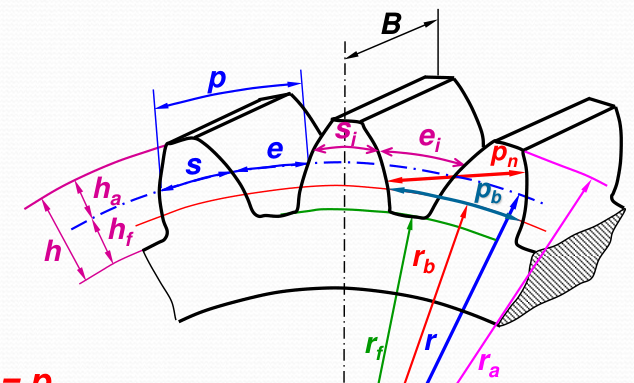
\includegraphics[width=7cm]{img/1.png}
            \end{figure}
\subsubsection{部分名称}
\begin{description}[leftmargin=1.5cm,style=nextline,nosep]% nosep没有垂直间隔
  \item[齿顶圆(above)] $d_a,r_a,h_a$
  \item[齿根圆] $r_f,d_f,h_f$
  \item[齿厚] $e_i$
  \item[齿槽宽] $s_i$
  \item[齿距] $p_i=e_i+s_i$
  \item[分度圆] $e_i=s_i$ 时候的圆,规定的计算基准圆  
  \item[齿全高] $h=h_a+h_f$
  \item[齿宽]$B$       
\end{description}
\subsubsection{基本参数}
记住以下五个基本参数:齿数,模数,分度圆压力角,齿顶高系数,顶隙系数。注意中心距不是基本参数。
\begin{description}[nosep]% nosep没有垂直间隔
  \item[齿数] $Z$
  \item[模数] $m$ (mm)
  \begin{align}
    l=\pi d= p z &\implies d=\frac{p}{\pi}z\\
    m&=\frac{p}{m}
  \end{align}
  \item[分度圆压力角] $\alpha$ 渐开线某一点的速度方向(切线)和其受力(和原点连线垂线)。
          \begin{figure}[H]
              \centering
              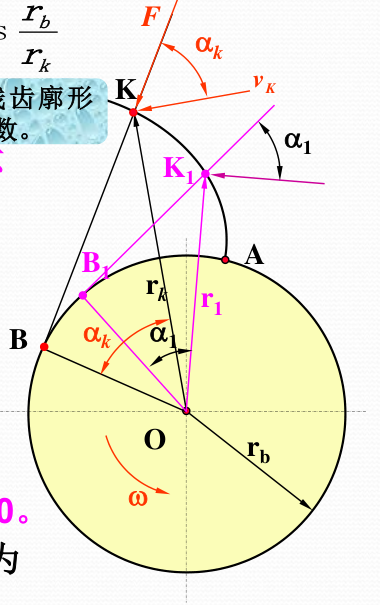
\includegraphics[width=4cm]{img/2.png}
              \end{figure}
  $$ \cos \alpha_k=\sin \angle{BKO}=\frac{BO}{BK}=\frac{r_b}{r_k} $$
  
  不同半径处$\alpha$ 还不一样。基,齿顶,分度圆的$r_k$ 分别为$r_b,r_a,r$
  \item[齿顶高系数] $h_a^*$
  \item[顶隙系数] $c^*$
\end{description}
\subsubsection{主要计算公式}
        \begin{figure}[H]
            \centering
            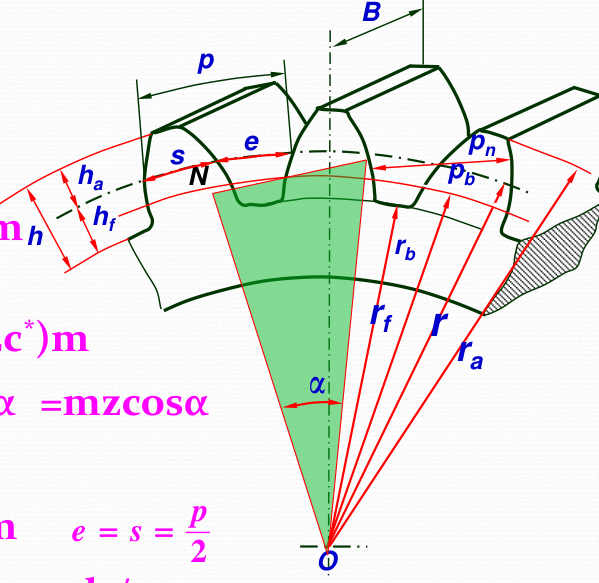
\includegraphics[width=6cm]{img/3.png}
            \end{figure}
\paragraph{对于直线:}
\begin{align*}
h_a&=h_a^*m\\
h_f&=(h_a*+c*)^*m\\
h&=h_a+h_f=(c^*+2h_a^*)\\
c&=c*m
\end{align*}

为什么规定齿根高要比齿顶高大呢?显然我不知道。

\textbf{并且对于正常齿,$1,0.25$。短,$0.8,0.3$。这个参数是你应该记住的,题目中有时候不会给出。你在算m的时候用的是分度圆的,但题目往往不会给出分度圆的。}


\paragraph{对于圆:}
\begin{description}[leftmargin=2.3cm,style=nextline,nosep]% nosep没有垂直间隔
  \item[分度圆直径] $d=mz$
  \item[齿顶圆直径] $d_a=d+2h_a=(z+2h_a^*)m$
  \item[齿根圆直径] $d_f=d\mathbf{-2h_f} =(z-2h_a^*-2c^*)m$  
  \item[基圆半径] $d_b=d\cos \alpha=mz\cos \alpha$ 
\end{description}

\paragraph{对于弧}
\begin{description}[leftmargin=2.3cm,style=nextline,nosep]% nosep没有垂直间隔
  \item[分度圆齿距] $m=\frac{p}{\pi}$
  \item[法向齿距] $p \cos \alpha$
\end{description}

\begin{quote}
{\qquad\parindent2\ccwd\kaishu\zihao{5}
对于内齿轮的话,$d_a=d-2h_a,d_f=d+2h_f$
}
\end{quote}
\paragraph{重要概念}
\begin{itemize}
\item 节圆的大小随中心距变化而变化。分度圆的大小只要齿轮加工好后就确定了
\item 分度圆的半径不能大于节圆的半径。
\item 分度圆:任一齿轮都有大小确定的分度圆。节圆:一对齿轮啮合时才存在,表明齿轮啮合特性
\end{itemize}
\end{document}